\section{Experiment}
\label{sec:experiment}
In this section, we will introduce the experimental settings and results. Our GPU device is Tesla P100 with 16GB memory. We use python 3.7 based Keras to implement all the experiments.

\subsection{Datasets and Baselines}
\label{sec:dataset}
The datasets of our experiment are  PHEME \cite{DBLP:conf/coling/KochkinaLZ18} and RumorEval\cite{DBLP:conf/semeval/EnayetE17}. These two datasets are widely used in the rumor detection research area. The details of PHEME are shown in Table.\ref{tab:pheme} and the details of RumorEval are shown in Table.\ref{tab:RumorEval}. The original PHEME contains 9 events and 4 of them are sparse, so we usually use PHEME-5 (following the existing works \cite{DBLP:conf/www/ChengNB20}). The PHEME-5 is formed by the top-5 scaled events, which contains 5802 threads and 1972 in them are rumors. 

To demonstrate the effectiveness of ART, we choose several baselines as a comparison, including Naive Bayes, SGD, FastText, Dense, BiLSTM, TextCNN, VRoC \cite{DBLP:conf/www/ChengNB20}, and some combinations of them. All the chosen baselines are contained in Table.\ref{tab:results_RE}. We use accuracy and micro-F1 as the evaluation metrics.

\begin{table}[htbp]
	\caption{PHEME}
	\centering
	\label{tab:pheme}
	\resizebox{0.8\linewidth}{!}{
		\begin{tabular}{|c|c|c|c|}
			\hline
			\textbf{Events} & \textbf{Threads} & \textbf{Tweets} & \textbf{Threads of Rumors}\\
			\hline
			Charlie Hebdo &2079&38268&458\\
			\hline
			Sydney siege  &1221&23996&522\\
			\hline
			Ferguson &1143&24175&284\\
			\hline
			Ottawa Shooting &890&12284&470\\
			\hline		
			Germanwings-crash&469&4489&238\\
			\hline
			\textbf{Total} & 5802 & 103212 & 1972 \\
			\hline	
		\end{tabular}
	}	
\end{table}

\begin{table}[htbp]
	\caption{RumorEval}
	\centering
	\label{tab:RumorEval}
	\resizebox{0.6\linewidth}{!}{
		\begin{tabular}{|c|c|c|c|}
			\hline
			\textbf{}  & \textbf{Threads} & \textbf{Branch} & \textbf{Tweets}\\
			\hline
			Development  &25&215&281\\
			\hline
			Testing  &28&772&1049\\
			\hline
			Training &272&3030&4238\\
			\hline	
			\textbf{Total}  &325 &4017 &5568 \\
			\hline		
		\end{tabular}
	}	
\end{table}


\subsection{Experimental Results}
The results on RumorEval are shown in Table.~{\ref{tab:RumorEval}}. The second column records the F1-Scores on each event, and "F, O, S, C, G" are the first chars of the corresponding event name. As we can see from the results, ART achieves the best performance on both average accuracy and average F1-Score. For each basic model, we can find the different results. TextCNN gets the best performance among these basic models. It is because the bag-of-words idea in TextCNN is suitable for the short text and various filters with different length effectively captures the features of key grams. Naive Bayes gets the worst performance. We think the reason is that the parameters in Naive Bayes are limited, which is not enough for this corpus. SGD+TextCNN achieves the best performance among the pairwise-added models. 

The results on PHEME are shown in Table.~\ref{tab:results_PHE}. It is shown that the ART model gets the second-best performance, which is a little lower than the combination of FastText, Dense, and TextCNN. We think it is because the scale of PHEME is larger than that of the RumorEval, and the SGD is not suitable for large-scaled dataset. Consequently, the worse performance of SGD pulls down the performance of ART. Also, the performance of basic models on PHEME proofs our explanation. The SGD gets the worst performance among all basic models. 

To sum up, the ART gets satisfactory performance on all datasets, which proved
the effectiveness.

\begin{table}[htbp]
	\caption{Results on RumorEval}
	\centering
	\label{tab:results_RE}
	\resizebox{1\linewidth}{!}{
		\begin{tabular}{|c|c|c|c|}
			\hline
			\multirow{2}{*}{\textbf{Methods}}  & \textbf{F1-Score on each event} & \multirow{2}{*}{\textbf{Average Accuracy}} & \multirow{2}{*}{\textbf{Average Micro-F1}}\\
			& \textbf{F, O, S, C, G} &  & \\
			\hline
			NB  & 0.937/0.924/0.907/0.929/0.617 & 0.910 & 0.863\\
			\hline
			SGD  & 0.977/0.964/0.942/0.928/0.927 & 0.950 & 0.948\\
			\hline
			FastText & 0.973/0.944/0.927/0.905/0.954
			& 0.938 & 0.940 \\
			\hline	
			Dense  & 0.964/0.951/0.939/0.937/0.919
			&0.946 &0.942 \\
			\hline
			BiLSTM  & 0.972/0.909/0.910/0.895/0.901
			&0.920 &0.917 \\
			\hline
			TextCNN  & 0.991/0.964/0.939/0.934/0.900
			& 0.953 & 0.946 \\
			\hline
			FastText + Dense  &0.979/0.951/0.936/0.918/0.964
			& 0.947 & 0.950 \\
			\hline
			FastText + TextCNN  & 0.975/0.940/0.925/0.898/0.954
			& 0.935 & 0.938 \\
			\hline
			SGD + TextCNN  & 0.979/0.964/0.942/0.935/0.927
			& 0.953 & 0.950 \\
			\hline
			Dense + TextCNN  & 0.964/0.954/0.945/0.926/0.88
			& 0.942 & 0.934 \\
			\hline
			FastText+ Dense + TextCNN  & 0.979/0.947/0.932/0.907/0.964
			& 0.942 & 0.946 \\
			\hline
			FastText+ SGD + TextCNN  & 0.977/0.955/0.941/0.925/0.937
			& 0.948 & 0.947 \\
			\hline
			VRoC \cite{DBLP:conf/www/ChengNB20}  &0.640/0.703/0.611/0.685/0.520
			& 0.644 & 0.632 \\
			\hline
			ART  &0.979/0.961/0.952/0.943/0.937
			& \textbf{0.956} & \textbf{0.955} \\
			\hline					
		\end{tabular}
	}	
\end{table}

\begin{table}[htbp]
	\caption{Results on PHEME}
	\centering
	\label{tab:results_PHE}
	\resizebox{1\linewidth}{!}{
		\begin{tabular}{|c|c|c|c|}
			\hline
			\multirow{2}{*}{\textbf{Methods}}  & \textbf{F1-Score on each event} & \multirow{2}{*}{\textbf{Average Accuracy}} & \multirow{2}{*}{\textbf{Average Micro-F1}}\\
			& \textbf{F, O, S, C, G} &  & \\
			\hline
			NB  & 0.976/0.926/0.888/0.900/0.735
			& 0.907 & 0.885\\
			\hline
			SGD  & 0.964/0.897/0.875/0.884/0.880
			&0.893&0.880\\
			\hline
			FastText &0.980/0.922/0.915/0.902/0.919
			&0.927&0.927\\
			\hline	
			Dense  & 0.977/0.912/0.905/0.891/0.913
			& 0.919 & 0.920 \\
			\hline
			BiLSTM  & 0.978/0.931/0.909/0.899/0.932
			& 0.927 & 0.930 \\
			\hline
			TextCNN  & 0.984/0.927/0.919/0.901/0.917
			& 0.930 & 0.930 \\
			\hline
			FastText + Dense  & 0.981/0.924/0.916/0.903/0.916
			& 0.928 & 0.928 \\
			\hline
			FastText + TextCNN  &0.984/0.928/0.923/0.910/0.927
			& 0.934 & 0.934 \\
			\hline
			SGD + FastText  & 0.981/0.925/0.913/0.904/0.913
			& 0.927 & 0.927 \\
			\hline
			Dense + TextCNN  & 0.986/0.894/0.926/0.908/0.930
			& 0.927 & 0.929 \\
			\hline
			FastText+ Dense + TextCNN  &0.987/0.935/0.925/0.918/0.930
			& \textbf{ 0.939} & \textbf{0.939} \\
			\hline
			FastText+ SGD + TextCNN  & 0.982/0.932/0.922/0.912/0.926
			& 0.934 & 0.935 \\
			\hline
			ART  &0.988/0.937/0.921/0.915/0.917
			& 0.936 & 0.935 \\
			\hline					
		\end{tabular}
	}	
\end{table}

\subsection{Different Embedding Strategies}
As introduced in section.\ref{sec:process_embedding}, there are several embedding strategies. To find the most proper embedding strategies, we conduct experiments to make a comparison of them. The existing work usually adopts the pre-trained embedding strategy. However, we find that the most proper embedding strategies are random embedding. We also add a self-trained embedding strategy into comparison.

The experimental results are shown in Table.~\ref{tab:embedding}. From the results, we can find that the random embedding strategy significantly outperforms the others on both average accuracy and average micro-F1. Self-trained embedding strategy achieves the second-best performance with a little superiority than that of the Google News Word2Vector. Moreover, we also test the GloVe embedding and the results are worse than Google News Word2Vector.

\begin{table}[htbp]
	\caption{Results of Different Embedding Strategies}
	\centering
	\label{tab:embedding}
	\resizebox{0.9\linewidth}{!}{
		\begin{tabular}{|c|c|c|c|}
			\hline
			\multirow{2}{*}{Events}  & \textbf{F1-Score on each event} & \multirow{2}{*}{\textbf{Average Accuracy}} & \multirow{2}{*}{\textbf{Average Micro-F1}}\\
			& \textbf{F, O, S, C, G} &  & \\
			\hline
			\multicolumn{4}{|c|}{\textbf{Google News Word2Vector}} \\
			\hline
			Dense  & 0.651/0.440/0.547/0.467/0.400
			& 0.542 & 0.501\\
			\hline
			BiLSTM  & 0.771/0.584/0.697/0.681/0.576
			&0.675&0.662\\
			\hline
			TextCNN  & 0.760/0.594/0.735/0.710/0.538
			& 0.689 & 0.667 \\
			\hline
			\multicolumn{4}{|c|}{\textbf{Self-trained Word2Vector}} \\
			\hline
			Dense  & 0.727/0.532/0.629/0.620/0.575
			& 0.635 & 0.616\\
			\hline
			BiLSTM  & 0.907/0.739/0.789/0.792/0.694
			&0.806&0.784\\
			\hline
			TextCNN  & 0.812/0.678/0.776/0.766/0.618
			& 0.757 & 0.730 \\
			\hline	
			\multicolumn{4}{|c|}{\textbf{Random Embedding}} \\
			\hline
			Dense  & 0.964/0.951/0.939/0.937/0.919
			& \textbf{0.946} &\textbf{0.942} \\
			\hline
			BiLSTM  & 0.972/0.909/0.910/0.895/0.901
			&\textbf{0.920} &\textbf{0.917} \\
			\hline	
			TextCNN  & 0.991/0.964/0.939/0.934/0.900
			& \textbf{0.953} & \textbf{0.946} \\
			\hline	
		\end{tabular}
	}	
\end{table}

\subsection{Details of Settings and Parameters}
In this part, we will introduce the detailed settings of the experiments. The chosen optimizer in the deep learning based model is Adam. The loss function is cross-entropy. We split the whole dataset into a proportion of 6:2:2. For a deep learning based model, we usually run it more than 50 epochs until convergence. Also, as shown in Fig.~\ref{fig:parameter}, we conduct various experiments to find the best parameters.

For simplicity, we only show the parameter adjustment on RumorEval as an example. We chose the embedding dimension, batch size, and hidden units as the representative parameters. During each running, we vary one parameter and fix the other parameters to record the variation trend of ART. The Fig.~\ref{fig:parameter_events} shows the results during parameter adjustment on each event. The Fig.~\ref{fig:parameter_art} records the performance of the ART during parameter adjustment. It can be seen that when the embedding dim is 32, batch size is 64, and hidden units is 100, the ART gets the best performance on RumorEval dataset. The smaller parameter value also corresponds to the small scale of RumorEval.

\begin{figure}[htbp]
	\centering
	\subfigure{
		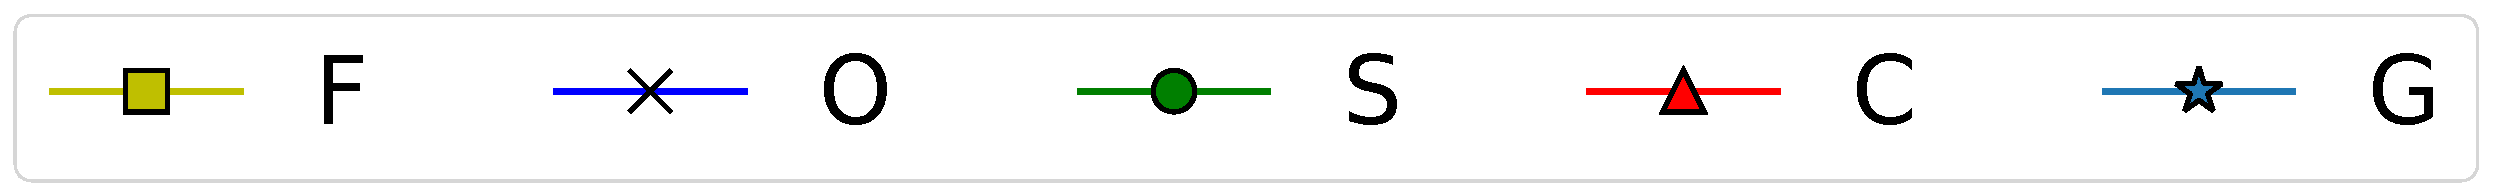
\includegraphics[width=0.4\linewidth]{fig/legend_f1}
	}
	\setcounter{subfigure}{0}
	\subfigure[Affects of Parameters on Different Events]{
		\label{fig:parameter_events}
		\begin{minipage}[b]{0.35\linewidth}
			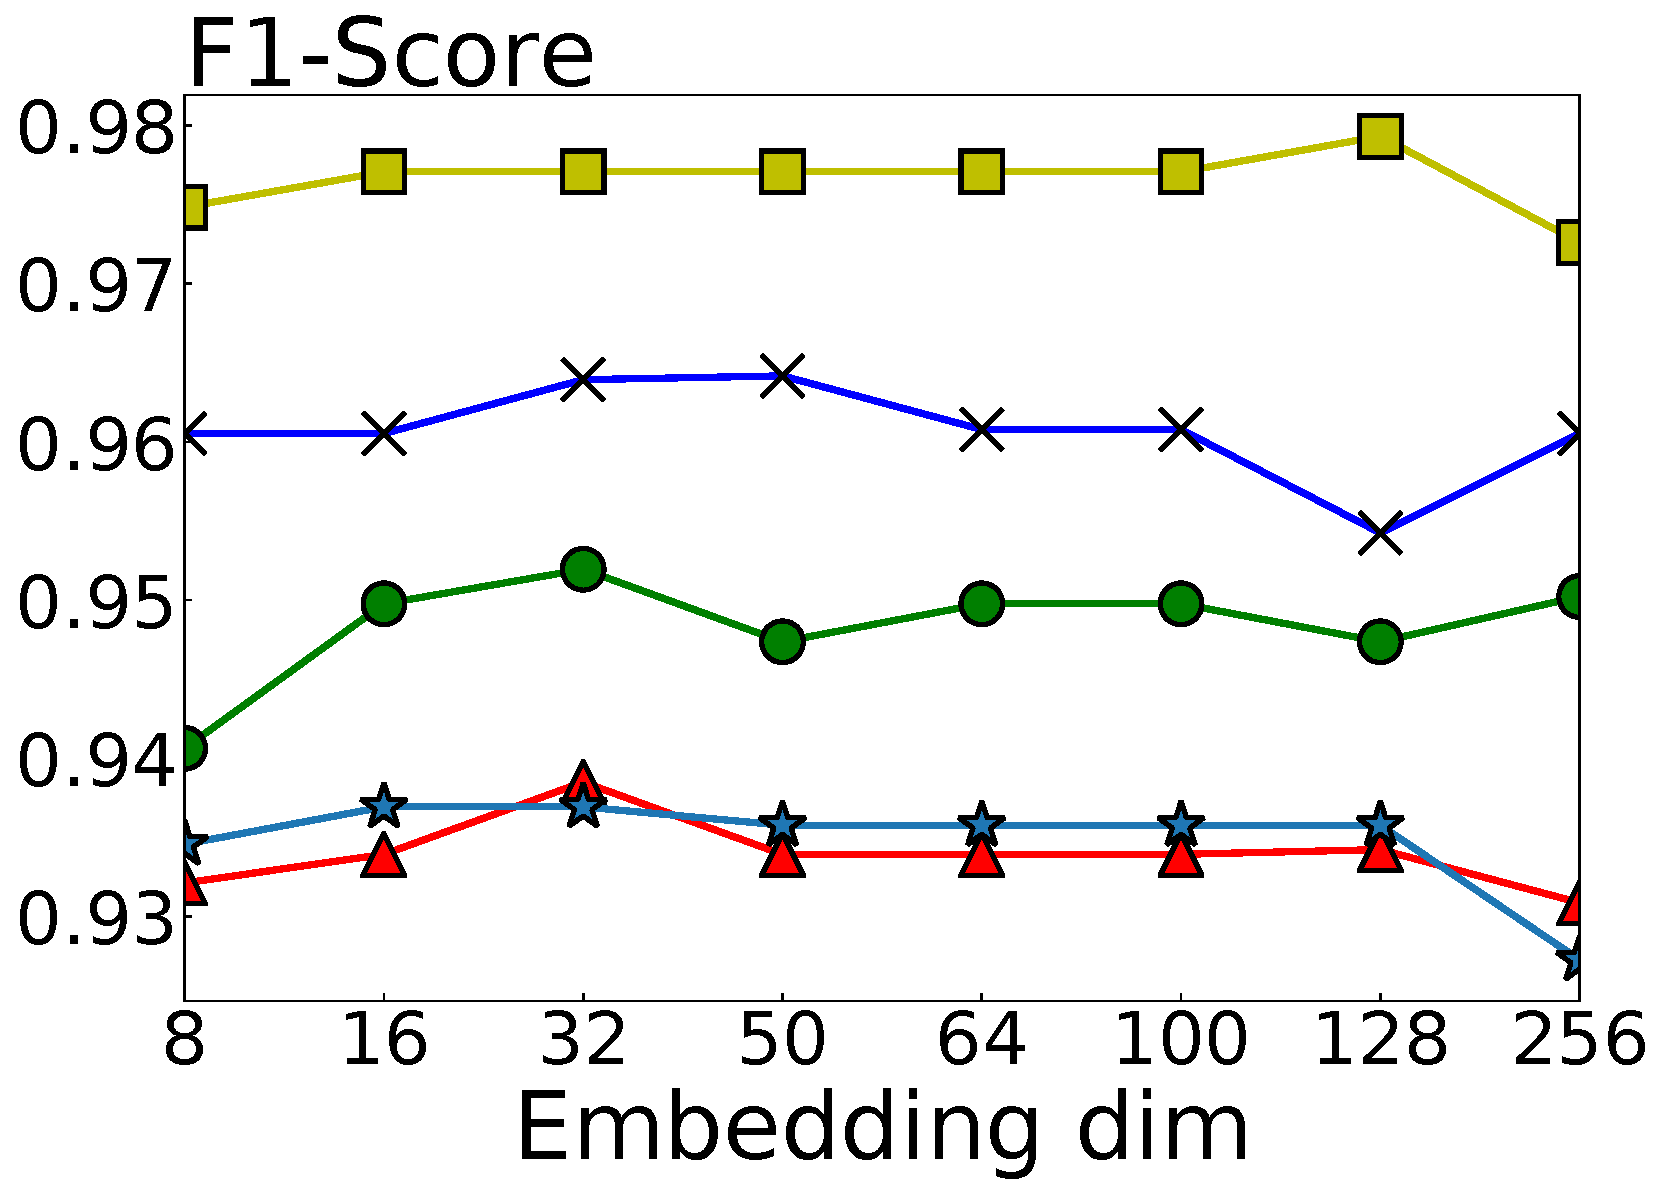
\includegraphics[width=1\linewidth]{fig/embedding_dim_events}
		\end{minipage}
		\begin{minipage}[b]{0.35\linewidth}
			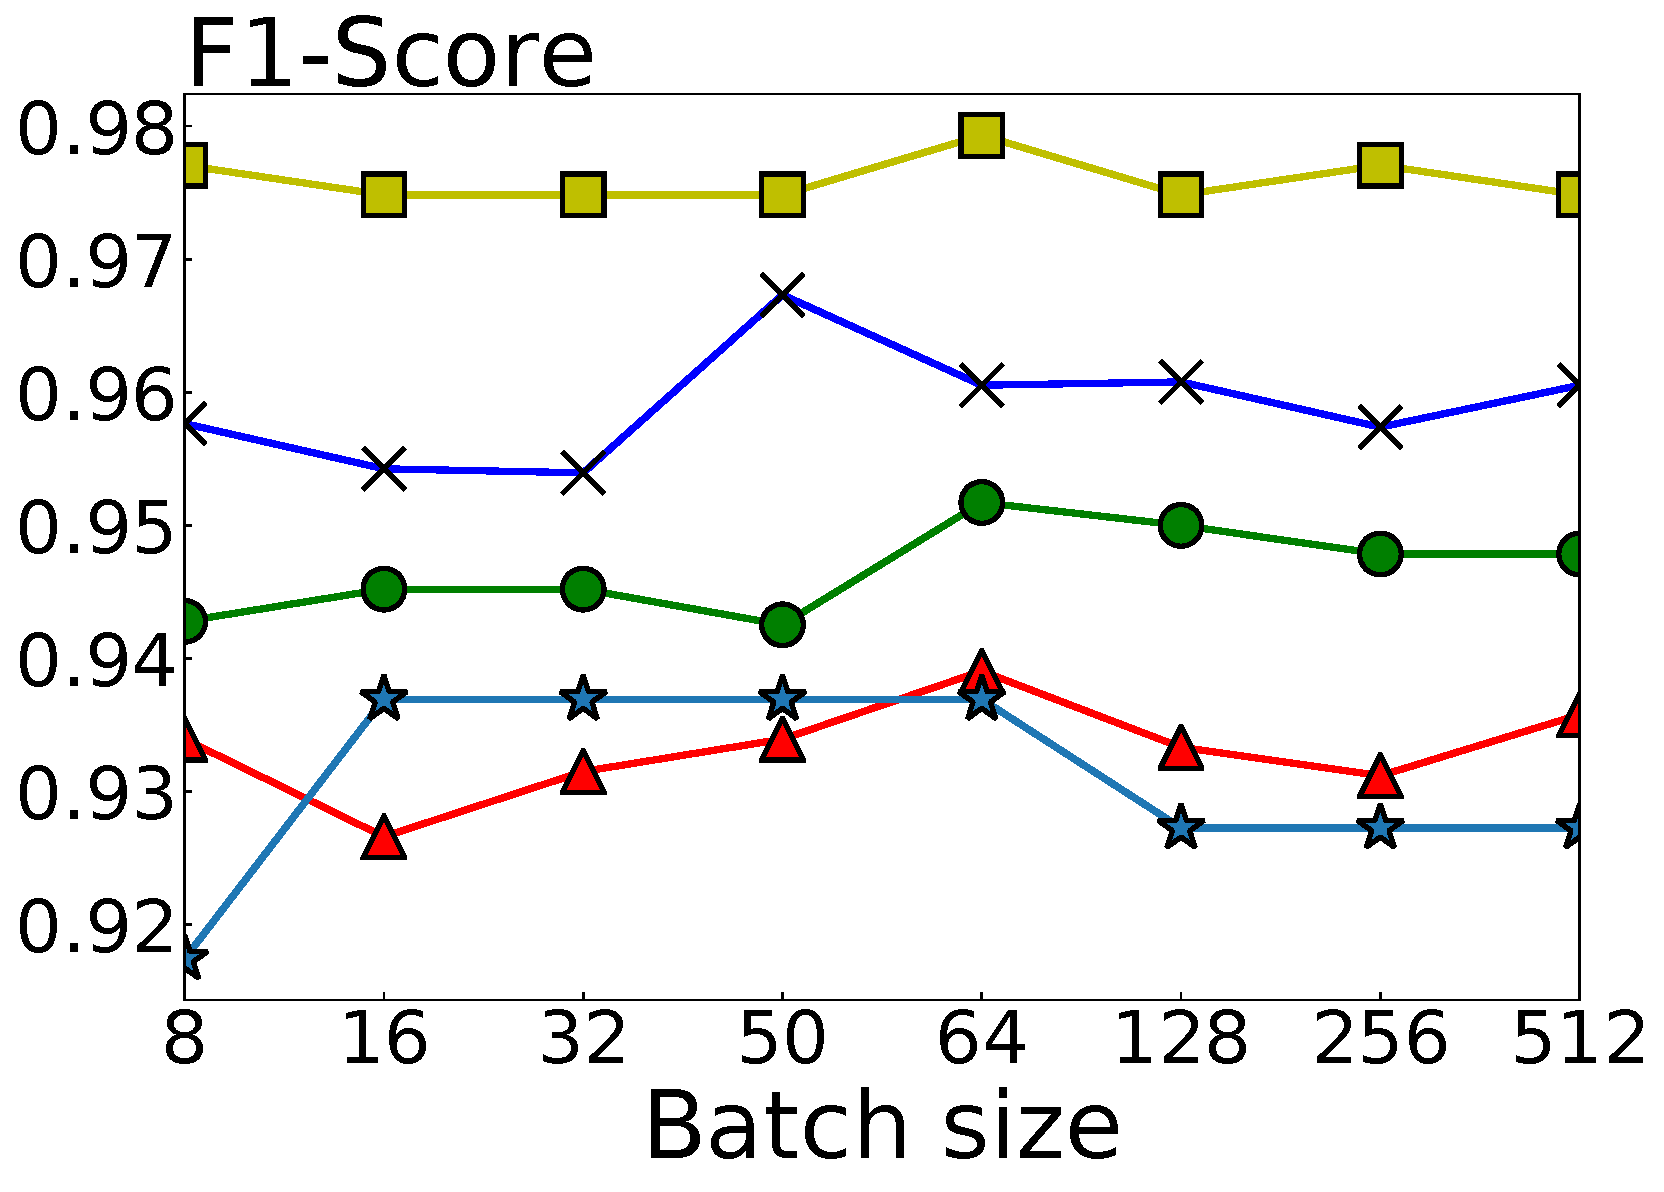
\includegraphics[width=1\linewidth]{fig/batch_size_events}
		\end{minipage}
		\begin{minipage}[b]{0.35\linewidth}
			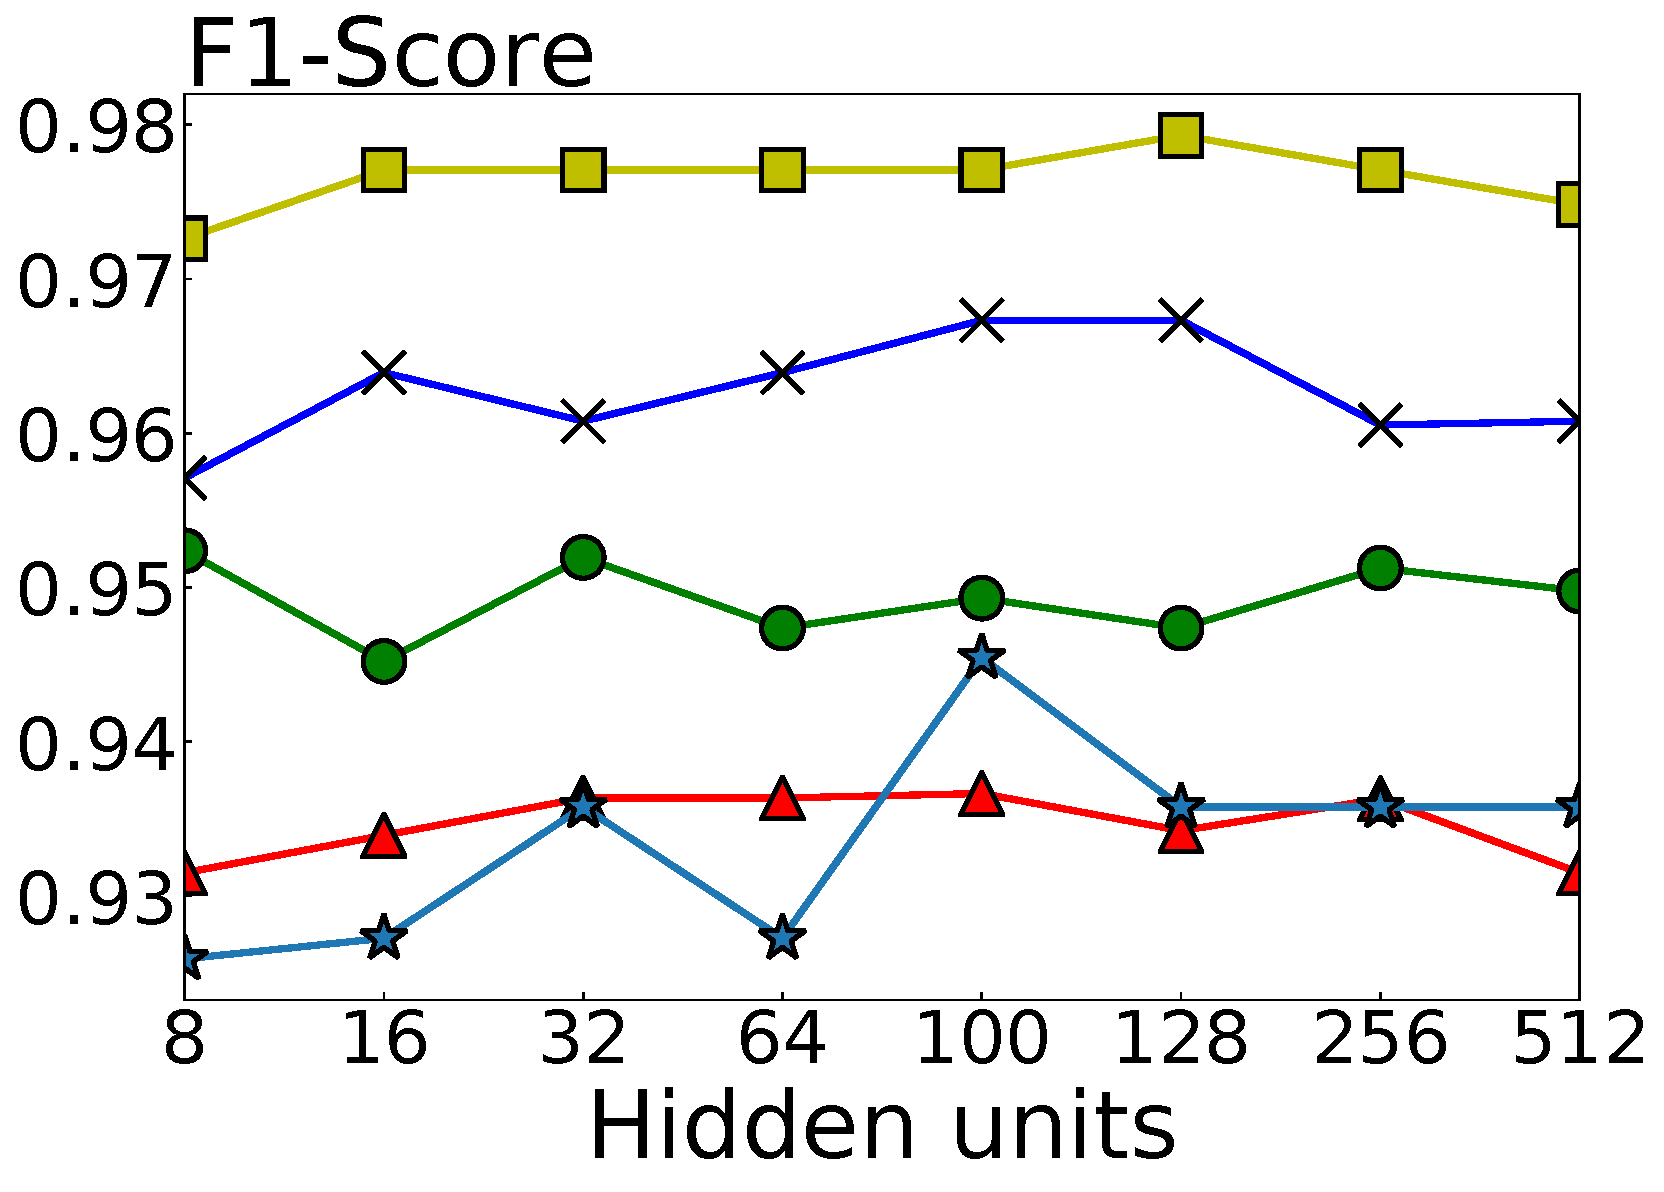
\includegraphics[width=1\linewidth]{fig/hidden_units_events}
		\end{minipage}
	}
	
	
	\subfigure{
		
\includegraphics[width=0.4\linewidth]{fig/legend_acc_macroF}
	}
	\setcounter{subfigure}{1}
	\subfigure[Affects of Parameters on F1-Scores and Accruancy]{
		\label{fig:parameter_art}
		\begin{minipage}[b]{0.35\linewidth}
			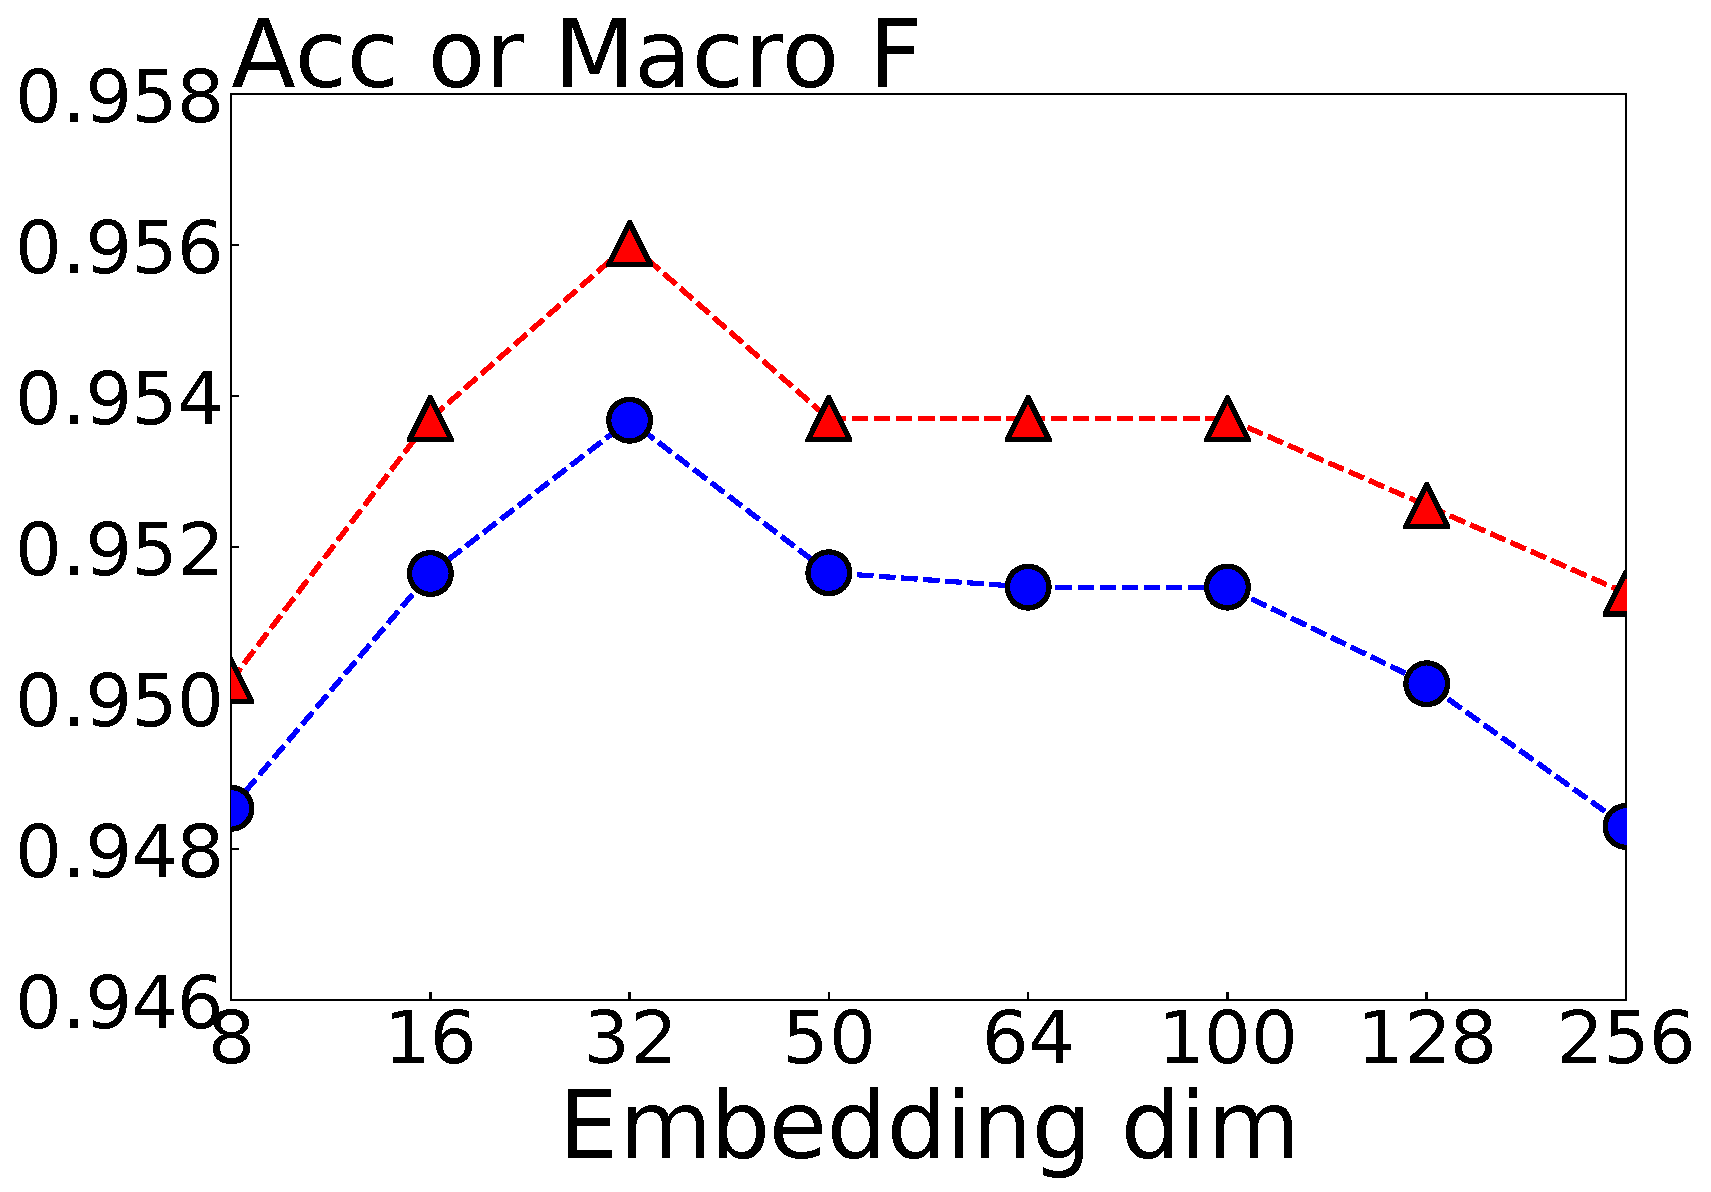
\includegraphics[width=1\linewidth]{fig/embedding_dim}
		\end{minipage}
		\begin{minipage}[b]{0.35\linewidth}
			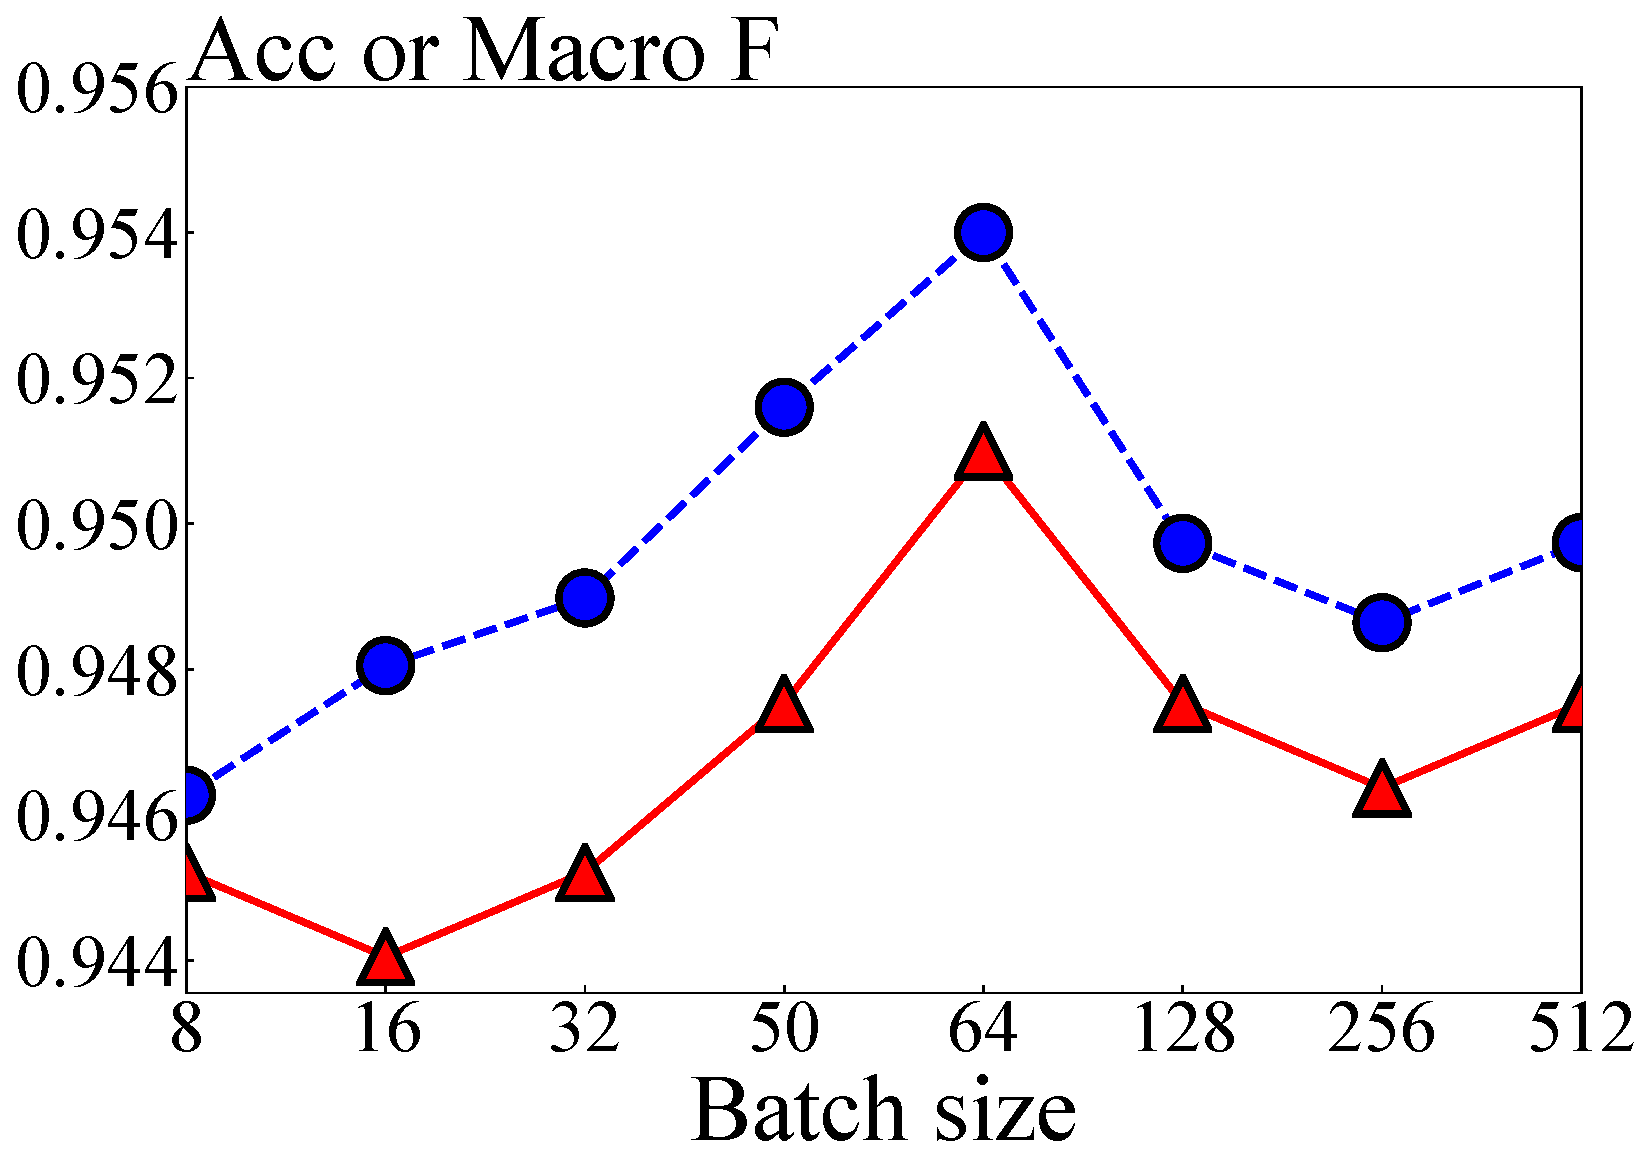
\includegraphics[width=1\linewidth]{fig/batch_size}
		\end{minipage}
		\begin{minipage}[b]{0.35\linewidth}
			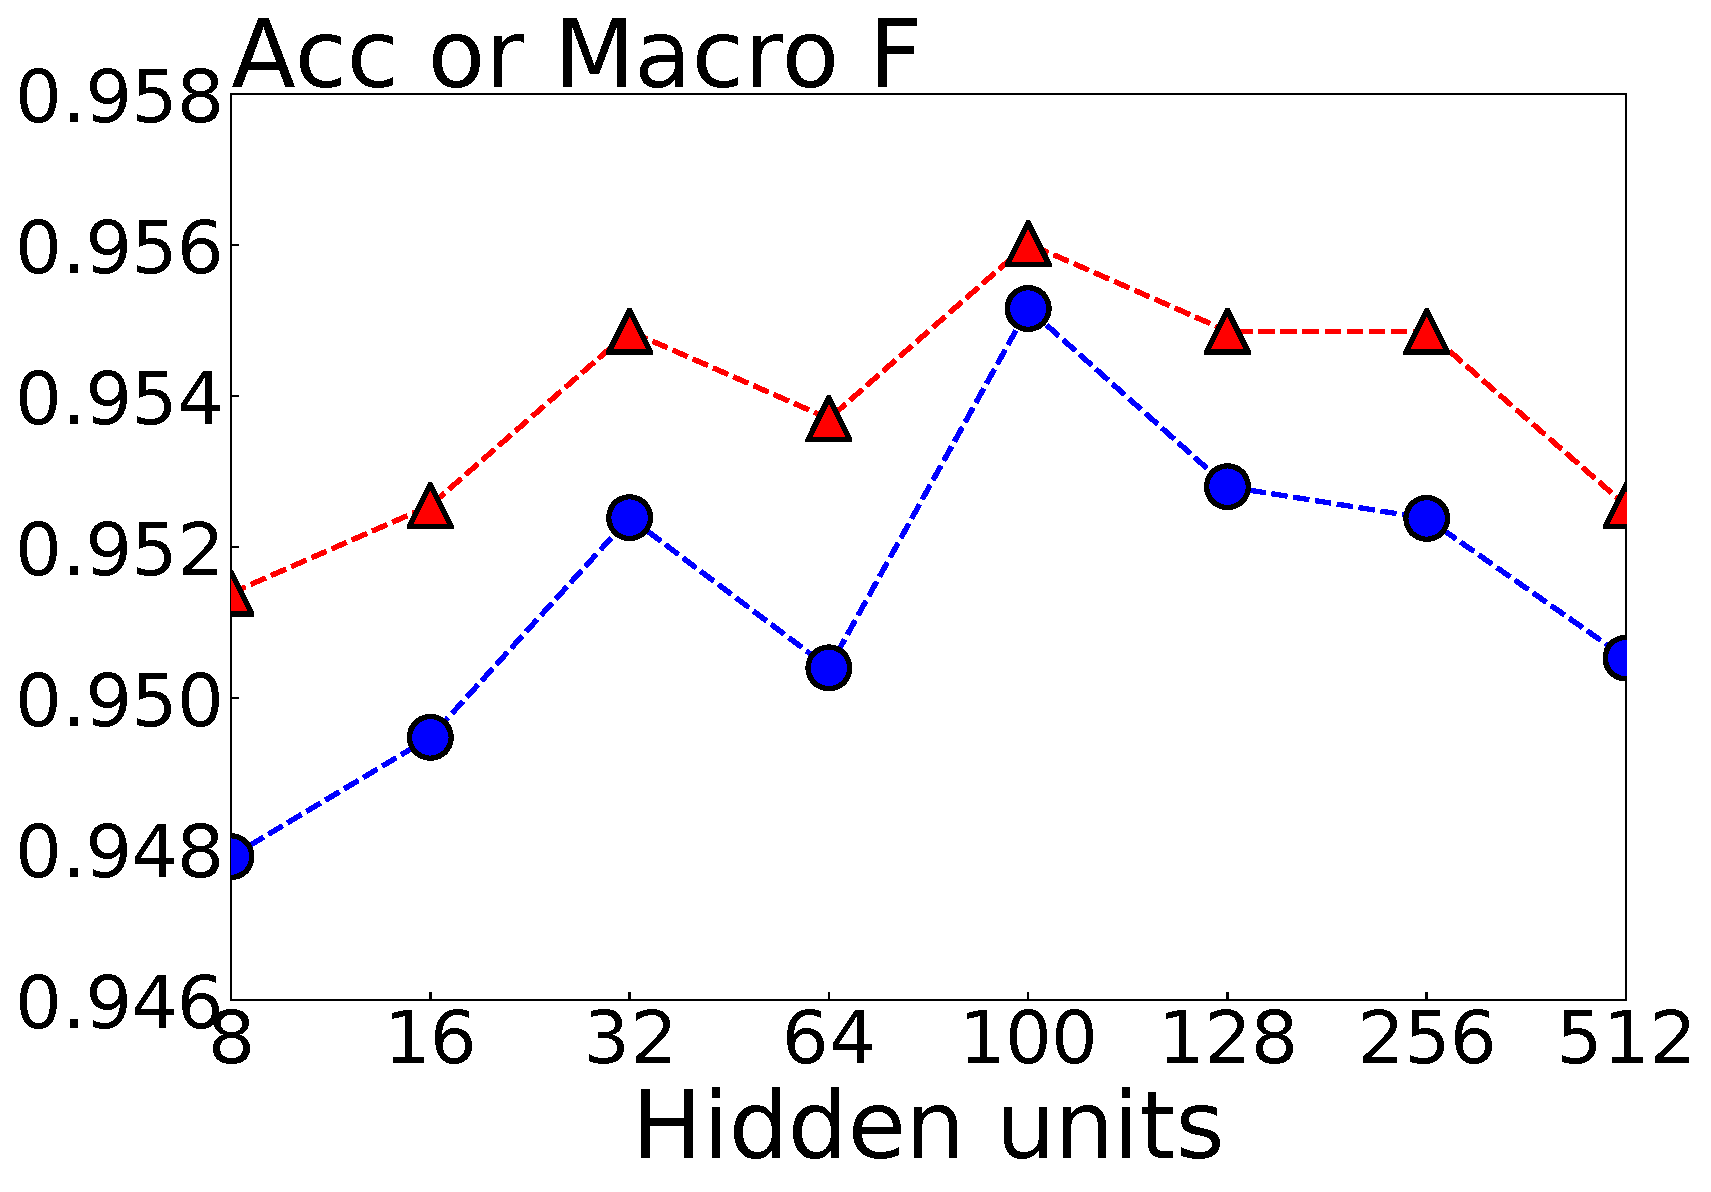
\includegraphics[width=1\linewidth]{fig/hidden_units}
		\end{minipage}
	}
	\caption{Adjustment of Parameters}
	\label{fig:parameter}
\end{figure}


\subsection{Discussions}
Rumor Tracking is a valuable sub-task of automatically rumor defeating. In this paper, we proposed an aggregated model named ART.  By adding specific features for rumor tracking and adopting a voting based aggregating strategy. We promote the performance of rumor tracking task on accuracy and F1-score. Also, well-designed experiments are carried out to demonstrate the effectiveness and efficiency of ART. Experimental results on benchmark datasets suggest that our model leads the baseline methods by over 5\% on average. In the feature, we will explore more efficient features for rumor detection, such as the links between users. Besides, we will explore a weighted voting strategy to optimize the aggregation. For instance, the weights can be learned from reinforcement learning on the rumor series.

